\documentclass{beamer}
\mode<presentation>{}
\usetheme{Warsaw}
\usepackage{hyperref}
\usepackage[super]{natbib}
\usepackage{graphicx}

\title{Harnessing the Power of \LaTeX}
\author{Karl Ahrendsen \and Andrew Vikartofsky}
\institute{University of Nebraska-Lincoln}
\date{\today}

\begin{document}

\begin{frame}
	\titlepage
\end{frame}

\section{What is \LaTeX?}
\subsection{\TeX}
\begin{frame}
	\frametitle{\TeX}
    \begin{itemize}
        \item A typesetting (or formatting) system
				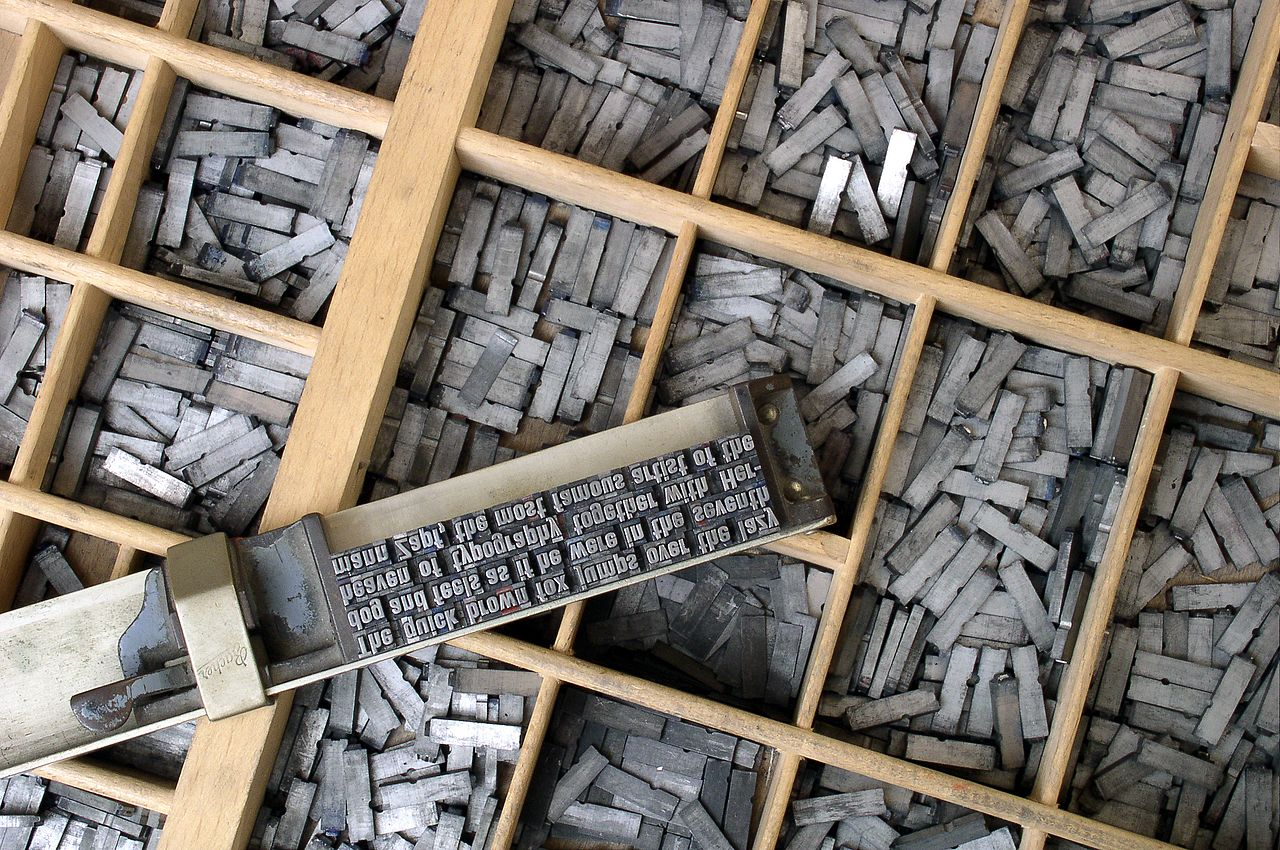
\includegraphics[width=50px]{img/metalWords.jpg}
				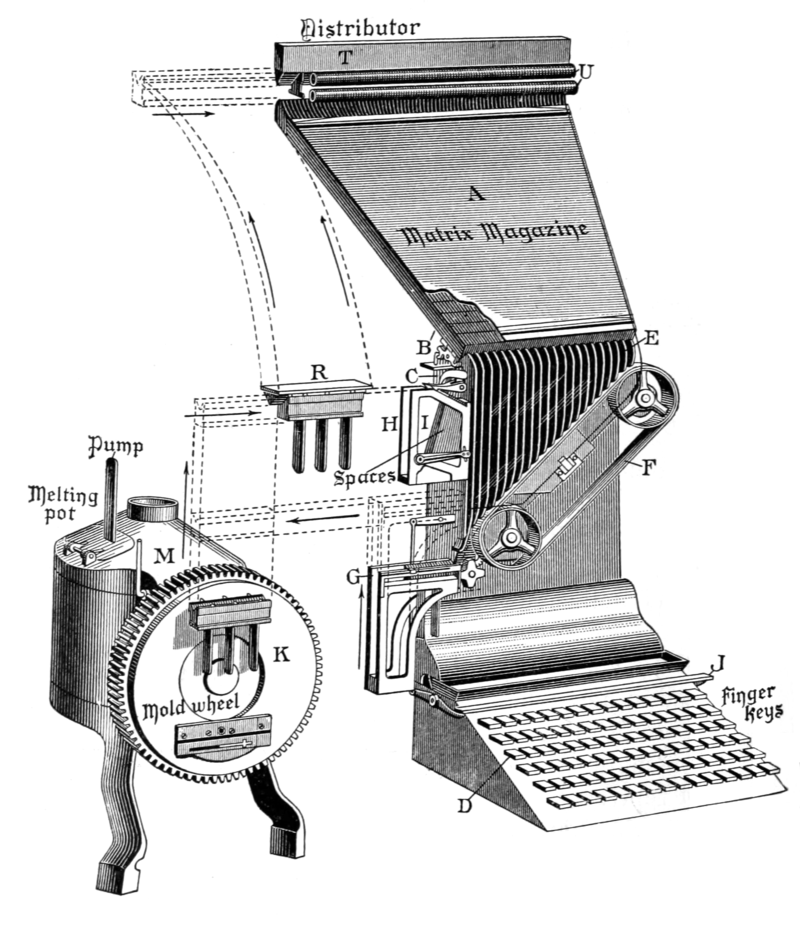
\includegraphics[width=50px]{img/typesettingMachine.png}
        \item Created by Donald Knuth
			% "Father of algorithm efficiency analysis"
        \item Provides precision typsetting for computers
		\item Designed with two goals~\cite{wikiTex}:
            \begin{itemize}
                \item Allow anybody to produce high-quality books with minimal effort.
                \item Provide a system that would give exactly the same results on all computers, at any point in time.
			\end{itemize}
    \end{itemize}
\end{frame}
\subsection{\LaTeX}
\begin{frame}
    \frametitle{\LaTeX}
    \begin{itemize}
            % Original author: Leslie Lamport
        \item Provides a high-level language to access the power of TeX
        \item A document preparation system
			\begin{itemize}
				\item Focus on content rather than formatting
				\item Writer uses plain text vs. formatted text (WYSIWYG)
			\end{itemize}
        \item Uses TeX to format its output
            % TeX handles layout, LaTeX Handles Content
    \end{itemize}
\end{frame}

\section{Why \LaTeX?}
\begin{frame}
	\frametitle{Why \LaTeX?}
    \begin{itemize}
		\item It might be necessary...
        \item Easy formatting of mathematical equations
        \item Cross referencing tools
		\item Modular documents
        \item It just looks sexy...
            % TeX handles layout, LaTeX Handles Content
    \end{itemize}
\end{frame}

\section{Basics}
\begin{frame}
	\begin{itemize}
		\item Only need to edit *.tex files
		\item Designate content with \textbackslash begin\{\}, \textbackslash end\{\}, and other labels
		\item Whitespace is (almost) meaningless
		\item Write, compile, review, repeat
		\item Previous documents and Google are your friend
	\end{itemize}
\end{frame}

\section{Workshop}
\begin{frame}
	\begin{itemize}
		\item ``The best way to learn is to do; the worst way to teach is to talk." -Paul Halmos
		\item Interactive demo document
	\end{itemize}
\end{frame}

\bibliographystyle{plain}
\bibliography{presentation}

\end{document}
